\section{Selected Algorithms}
\label{sec:algorithms}

Guided by~\cite{rahate}, five algorithms in total were chosen to be used in providing the basis for evaluating the languages under scrutiny. Of the five, four are exact-matching algorithms and one is an approximate-matching algorithm. One algorithm matches multiple patterns in a single examination of a sequence, while the remaining algorithms match only single patterns.

In this section, these algorithms are introduced and the first four briefly explained. The fifth algorithm will receive a more in-depth treatment due to it being a new approach. An understanding of the underlying mechanics of the algorithms will be helpful when later evaluating their implementations.

During the process of running experiments and analyzing the results, it was decided to add a variation of the fifth algorithm to the existing set. As a variation, it is not covered in the same depth as the fifth and original algorithm is. Instead, it is dealt with in greater detail in section~\ref{subsubsec:dfa_regexp}.

\subsection{Knuth, Morris, and Pratt}

The Knuth-Morris-Pratt~\cite{knuth} algorithm is one of the foundational algorithms in the area of string matching and text searching. It is still used in the present day, with implementations as recent as the Rust-Bio project~\cite{rust}. This was chosen primarily for historical significance, but also for ease of implementation.

Knuth-Morris-Pratt is an \textit{exact matching} algorithm, meaning that it matches the desired pattern exactly or not at all. It finds all instances of the pattern within the target string, including overlapping instances, in time-complexity linear to the sum of the pattern length and the target length.

\begin{figure}[ht]
    \centering
    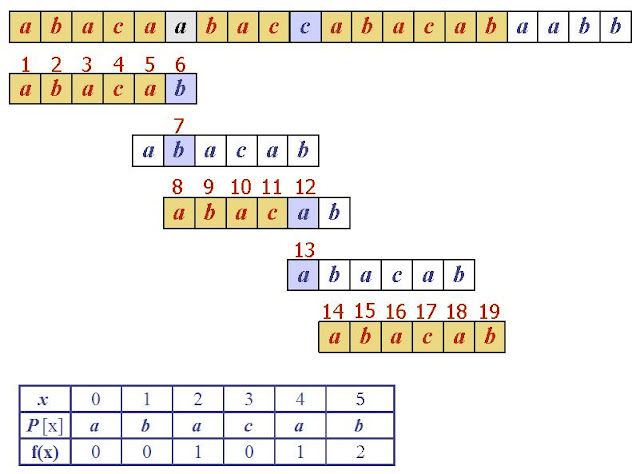
\includegraphics[width=0.65\textwidth]{figures/kmpexample.jpg}
    \caption[Example of Knuth-Morris-Pratt algorithm]{Example of Knuth-Morris-Pratt (original source~\cite{shandilya})}
    \label{fig:image:kmpexample}
\end{figure}

Generally when matching, the pattern is aligned with positions in the target string. Shifting is done when a character mismatch is found between an index in the target and the corresponding index in the pattern. Where a naive implementation might shift the pattern by one place after each failed match, resulting in a time complexity approaching O($mn$), the Knuth-Morris-Pratt approach is built on the concept of an auxiliary table (referred to as the ``next'' table) that instructs the matching algorithm on how much to shift the pattern over the target stream. Based on repetition within the pattern itself, the table may call for a shift of the pattern by more than one character for a given mismatch.

The computation of this table is shown in the paper to require O($m$) steps, and the process of matching the pattern to the target takes at most an additional $2n$ steps. This is due to the fact that, at each step of the matching process, only one of the text pointer or the pattern pointer are moved (each of which can only move $n$ times at most). This results in a worst-case run-time bounded by O($m+n$).

As an example, consider a search for the pattern ``CTAGC'' in a sequence that starts with ``CGCCTAGCG''. The first step is to compute the ``next'' table according to the algorithm, shown in figure~\ref{fig:kmp_next}.

\begin{figure}[ht]
\centering
\input{figures/kmp-next}
\caption{Knuth-Morris-Pratt next-table}
\label{fig:kmp_next}
\end{figure}

With the table in hand, the process moves to matching. The matching algorithm goes through the following steps:

\begin{enumerate}
\item $i$ and $j$ both initialize to 0
\item $p_0 = s_0$, so $next$ is not consulted
\item $i$ and $j$ increment, both to 1 and 1
\item $p_1 \neq s_1$, so $i = next[1]$ and becomes 0
\item $p_0 \neq s_1$, so $i = next[0]$ and becomes -1
\item $i$ and $j$ increment, to 0 and 2 respectively
\item $p_0 = s_2$, so $next$ is not consulted
\item $i$ and $j$ increment
\item $p_1 \neq s_3$, so $i = next[1]$ and becomes 0
\item $p_0 = s_3$, so $next$ is not consulted
\item $i$ and $j$ increment
\item $p_i$ continues to match $s_j$ as both variables increment. When $i = 5$, the algorithm detects a match.
\end{enumerate}

Here, the Knuth-Morris-Pratt algorithm has found the match in 10 character comparisons, 5 of which were required to verify the full match.

\subsection{Boyer and Moore}

In the same year that Knuth, Morris and Pratt published their paper, Boyer and Moore published as well~\cite{boyer}. This algorithm is also an exact matching approach, that is based on the research of Knuth, et al. The Boyer-Moore performance improvements are based on searching from the end of the pattern rather than the beginning, and computing two tables to use in optimizing the jumps through the sequence string when mismatches are discovered. This algorithm was chosen as an example of refinement and improvement of another sample algorithm.

Boyer and Moore postulated that, ``more information is gained by matching the pattern from the right than from the left.'' For example: If the target character that corresponds to the current location of the last character from the pattern is not only a mismatch but also does not appear in the pattern at all, the pattern may then be shifted right by its full length. They refer to this algorithm as being ``usually sublinear,'' meaning that when finding the location of the pattern within the target the number of compared characters is usually less than $i+m-1$ (where $m$ is the pattern length and $i$ is the position within the target where the match of the pattern begins).

The first of the two tables is the simplest to compute. It is the size of the alphabet of the pattern and sequence\footnote{In these implementations, to avoid constantly translating the four characters into values between 0 and 3, the alphabet-size was set to 128 for convenience.}, and it tracks the number of positions by which the pattern can be moved down the sequence without additional checking for matches. Boyer and Moore define each entry in this table as being $m$ (the pattern's length) when the character does not appear in the pattern at all, and $m - i$ otherwise (where $i$ is the right-most index within the pattern where the character does occur). Using the same example pattern and sequence as in the previous section, the first table (referred to as $delta_1$ in the paper and $bad\_char$ in the implementations) is shown in figure~\ref{fig:bm_bad_char}. Only the entries for the four characters that appear in patterns are shown.

\begin{figure}[ht]
\centering
\input{figures/bm-bad-char}
\caption{Boyer-Moore $delta_1$ table}
\label{fig:bm_bad_char}
\end{figure}

The second table (referred to as $delta_2$ in the paper and $good\_suffix$ in the implementations) is more complex to calculate, as it first requires calculation of suffixes within the pattern. In the paper, it is described as the distance that the pattern can be slid down in order to align the discovered sub-match (in the target) with the last $m - j$ characters of the pattern (where $j$ is the index within $delta_2$), plus the additional distance that the pointer within the target must be moved so as to restart the matching process at the right end of the pattern. This table is shown in figure~\ref{fig:bm_good_suffix}.

\begin{figure}[ht]
\centering
\input{figures/bm-good-suffix}
\caption{Boyer-Moore $delta_2$ table}
\label{fig:bm_good_suffix}
\end{figure}

When using the two tables to select the amount to shift, it is possible that the $delta_1$ table's value may be negative. Because of this a $max$ operator is applied to the two potential values and the largest possible shift is chosen. With both tables computed, the matching process begins with the pattern aligned to the starting character of the target string. The algorithm then goes through the following steps (where $m$ is the pattern length and $n$ is the sequence length):

\begin{enumerate}
\item $j$ (the pointer within the sequence) initializes to 0
\item $i$ (the pointer within the pattern) is set to $m - 1$ (4)
\item $p_4 \neq s_4$, so the tables are consulted
\item $delta_2(4)$ is 1, and $(delta_1(T) - m + 1 + i)$ = 3
\item $j$ advances by 3
\item $i$ is set to $m - 1$ (4)
\item $p_4 = s_7$, so $i$ is decremented
\item $p_i$ continues to match $s_{i+j}$ until $i$ becomes -1
\item A match is recorded and $j$ advances by $delta_2(0)$, to 7
\end{enumerate}

While the Knuth-Morris-Pratt algorithm had made 10 character comparisons to find the match, Boyer-Moore makes only 6, 5 of which were required to verify the match.

\subsection{Bitap}

The Bitap algorithm (sometimes known as ``Shift-Or'', or ``Shift-Add'') was initially developed by B\'{a}lint D\"{o}m\"{o}lki in 1964. In 1989 it was re-invented by Ricardo Baeza-Yates and Gaston H. Gonnet, and published in~\cite{baeza} in 1992. Here, it has been chosen for the distinctive approach when compared to the other algorithms.

In terms of time complexity, the algorithm is on the same terms as the previous ones, having a preprocessing time of O($m+\sigma$) (the length of the pattern plus the size of the alphabet) and a running time of O($n$). However, the operations it performs are all bit-oriented: shifts, complements, bitwise-and and bitwise-or. This resulted in this algorithm running significantly faster than either of Knuth-Morris-Pratt or Boyer-Moore on the experiment input data.

The structure of the algorithm is based on encoding the pattern in a vector of bitmaps. The vector has length equal to the alphabet size, and each element of the vector is a bit-field of width $W$, where $W$ is the size in bits of an unsigned integer. $W$ also limits the length of the pattern in this implementation, though it is possible to implement the algorithm for longer patterns.

The vector is initialized in the preprocessing phase first to an all-1's value in each slot, and then modified through a single pass over the pattern. For each character in the pattern, the slot corresponding to that character has the bit that corresponds to the pattern position flipped to 0. The resulting vector fully encodes the pattern. Using the example pattern from the previous two algorithms (``CTAGC''), imagine that the elements of the vector ($S$) are exactly as wide as the pattern (5 bits) and that there are only the four elements corresponding to the restricted alphabet of the pattern. This is shown in figure~\ref{fig:bitap_s_positions}.

\begin{figure}[ht]
\centering
\input{figures/bitap-s-positions}
\caption{Bitap shift positions vector}
\label{fig:bitap_s_positions}
\end{figure}

Here, it is clear that the letter ``C'' appears twice in the pattern as there are two 0-values in S(C). Each of the other three letters appear just once. Examining the bits of each S-value shows exactly where each letter appears in the pattern.

During the process of computing the $S$ vector, a ``limit'' value is also calculated: it starts out as 0, and has a number of bits set equal to the full width of the pattern. At the end of the loop that calculates $S$, the value of $limit$ is shifted to the right by one bit, then subjected to a bit-complement operation. The result is a value that can be directly used in comparison, when determining if a match has been found.

The process of searching for a match begins with a $state$ value of $W$ bit-width, set to all 1's. The target string is read one character at a time. For each iteration of this loop, $state$ is shifted to the left one bit (introducing a 0) and then \texttt{or}'d with the $S$ value of the character under the index. If, after this operation (the ``shift-or''), the value of $state$ is less than the value of $limit$ then a match has been found and will be reported.

\begin{figure}[ht]
\centering
\input{figures/bitap-matching}
\caption{Bitap matching process}
\label{fig:bitap_matching}
\end{figure}

Figure~\ref{fig:bitap_matching} shows the process of matching the example pattern to the same sequence used in previous algorithm examples. The $j$ column indicates the index of the character in the sequence, $s_j$ is the character at $j$, and $S(s_j)$ is the $S$-value for that character. The $state$ column shows the value of that variable at each iteration, while the ``result'' column shows the value of $state$ after the \texttt{or}-operation. Not shown is the $limit$ value, which in this example is \texttt{10000} (16 decimal). On the row where $j = 7$, we see that the high bit of $state$ is a 0 for the first time. This signals a match ($state < limit$), and the matching index is $j - m + 1$, or 3.

In this example the Bitap algorithm found the match after 8 rounds of the shift-or operation. No direct character-level comparisons were made, nor were any equality comparisons made. The process of finding the match involved only the two bit-level operations and a single ``less-than'' comparison for each iteration of the main loop.

\subsection{Aho and Corasick}

Alfred V. Aho and Margaret J. Corasick published their algorithm for searching multiple patterns at once in 1975~\cite{aho}. In their algorithm, a finite number of patterns are merged into a single deterministic finite automaton (DFA) which can then be applied over any number of target strings. The DFA is capable of finding all locations of all patterns in the set, with overlapping, in a single pass through the target string. This makes the algorithm significantly faster than the others for the simple reason that Aho-Corasick scans each target string once, regardless of the number of patterns. By contrast, each of the single-pattern algorithms scans the target string once per pattern. The choice of this algorithm was driven by an interest in comparing a multi-pattern algorithm to the single-pattern options, and an interest in exploring the use of a finite automaton for the matching process.

Aho and Corasick designed the pattern matching machine as a collection of three functions:

\begin{itemize}
\item A ``goto'' function $g$, which maps transitions from one state to the next based on the character being examined
\item A ``failure'' function $f$, which maps a state into another state whenever $g$ reports that there is no transition for the current state and current character
\item An ``output'' function $output$, which maps states to sets of patterns matched at the specific state
\end{itemize}

Construction of these three functions is accomplished through two supporting algorithms. The first fully constructs $g$ and partially computes $output$. The second fully constructs $f$ and completes the computation of $output$. The first algorithm takes only the set of patterns (referred to there as $K$) as input, while the second algorithm takes the resulting $g$ and $output$ from the first as input.

For an example, let $K$ be the list $\left\lbrace ACTG,~CTG,~AAGT \right\rbrace$. Constructing $g$ by the algorithm given in the paper yields the DFA given by the figures~\ref{fig:ac_goto_function} through~\ref{fig:ac_output_function}.

\begin{figure}[ht]
\centering
\input{figures/ac-goto-function}
\caption{Aho-Corasick goto function}
\label{fig:ac_goto_function}
\end{figure}

Starting with figure~\ref{fig:ac_goto_function}, the goto function $g$ provides the finite-state machine that lays out the transitions between states based on the character under consideration. Any state that does not have a transition for a given character is assumed to ``fail'' on that character, which is where the failure function $f$ comes into use. While it is given in the algorithm that there are no failure transitions for state 0, this is made explicit in the figure by including a self-referencing transition for ``G'' and ``T''.

\begin{figure}[ht]
\centering
\input{figures/ac-failure-function}
\caption{Aho-Corasick failure function}
\label{fig:ac_failure_function}
\end{figure}

In figure~\ref{fig:ac_failure_function}, the failure function $f$ shows how the processing of the DFA may jump around to implement a form of back-tracking. State 2 will move to state 5 on a failure transition, reflecting that the character previous to the state (``C'') could instead be the start of matching the ``CTG'' pattern. Because there are no failing transitions in state 0, that state is not represented in the figure.

\begin{figure}[ht]
\centering
\input{figures/ac-output-function}
\caption{Aho-Corasick output function}
\label{fig:ac_output_function}
\end{figure}

In figure~\ref{fig:ac_output_function}, the $output$ function is represented as an indexed array of sets. Most states (including state 0) have the empty set as output. The non-empty sets represent the found patterns by their index in the original list. State 10 has only a value of 2, representing the pattern ``AAGT''. Of note is state 4, whose set includes both the index 0 and the index 1. This reflects the fact that the three characters of pattern 1 overlap the last three characters of pattern 0.

To illustrate the process of this algorithm, consider the target string that begins with the sequence ``AACTG...''. Figure~\ref{fig:ac_progression} shows the progression of states as the pointer advances through the first five characters.

\begin{figure}[ht]
\centering
\input{figures/ac-progression}
\caption{Example of Aho-Corasick state progression}
\label{fig:ac_progression}
\end{figure}

Starting at the 0 state, the first ``A'' moves the DFA to state 1 after which the second ``A'' moves it to state 8. From 8, the character ``C'' is a failure transition, so the value of $f(8)$ is read. The value is 1, so the DFA immediately moves to state 1 and looks for a transition on ``C''. It exists, and the DFA moves to states 2, 3 and 4 in turn. Upon reaching state 4 the value of $output(4)$ is found to not be the empty set, so the machine signals a match of the patterns ``ACTG'' and ``CTG''.

Here, the Aho-Corasick algorithm has positively identified the presence of two of the three patterns encoded by the DFA. Only 5 characters from the target string were processed, and because the DFA indexes by the ordinal values of the characters no direct comparisons were made. Further, no back-tracking was required to find the second pattern.

\subsection{Approximate Matching with Gaps}
\label{subsec:dfa_gap}

For the fifth algorithm in the suite of experiments, it was decided to implement an approximate-matching algorithm. In this case, the algorithm chosen is a new algorithm that takes a different approach to approximate-matching: building a DFA with additional states that allow for measured gaps between the characters of the pattern.

The idea of using a DFA to represent the pattern is inspired primarily by~\cite{aho} and~\cite{becchi}. Becchi and Crowley, in particular, address the problem of representing the concept of \textit{counting} states in an extended definition of a finite automaton. In their work, they put forward a means of having special states that track the number of times they've been entered in sequence, only allowing exit from the state when the given number (count) of visits is satisfied.

From this, a different type of approximate-matching can be pictured: one that allows for well-defined, finite ``gaps'' between elements of the pattern being matched. Given a value $k$ that is a positive integer, gaps that are up to $k$ characters in length can be tolerated while still regarding the pattern as matching a point in the target sequence. And when $k = 0$, the approach becomes the naive exact-matching approach that is of time-complexity O($mn$).

Current algorithms for approximate matching in DNA sequences use a variety of approaches, such as edit distance. But methods based on edit distance can result in all changes or differences being clumped together as opposed to distributed across the pattern in a more balanced fashion. For example, given the same ``CTAGC'' pattern used for the previous single-pattern algorithms and $k = 3$ this algorithm would allow as many as 12 additions to the pattern in order to match a position in the sequence. Simply allowing an edit distance of 12 in a different algorithm could potentially lead to 12 additions being made between just two of the pattern characters. The algorithm described here is designed to prevent such uneven distribution of the gap letters in the matched segment of the sequence.

The basis of the algorithm is the notion that such an approximate match as described here can be expressed in terms of a regular expression that supports the specification of ranges of matches for a given class or symbol in the expression. Such a specification is generally encoded as \texttt{$\lbrace a,b \rbrace$} in an expression, where $a$ and $b$ are integers and $b \geq a$. Most compatible engines support several variant forms of this:

\begin{description}
\item[\texttt{$\lbrace a \rbrace$}:] matches exactly $a$ occurrences
\item[\texttt{$\lbrace a, \rbrace$}:] matches at least $a$ occurrences, with no upper limit
\item[\texttt{$\lbrace ,b \rbrace$}:] matches at most $b$ occurrences, with as few as zero
\item[\texttt{$\lbrace a,b \rbrace$}:] matches at least $a$ occurrences and at most $b$ occurrences
\end{description}

Using the fourth construct and the ``CTAGC'' pattern, an example regular expression for a value of $k = 3$ could look like:

\begin{center}
\texttt{C.$\lbrace 0,3 \rbrace$T.$\lbrace 0,3 \rbrace$A.$\lbrace 0,3 \rbrace$G.$\lbrace 0,3 \rbrace$C}
\end{center}

However, this not correct because the dot (``\texttt{.}'') matches all characters. This is not desirable, as any ``T'' encountered after the initial ``C'' should move to that part of the pattern rather than possibly being subsumed by the dot. Additionally, in a general regular expression engine the dot will match \textit{all} characters, including those not part of the DNA alphabet. Restricting the counting-states to just the alphabet of the problem, and eliminating the target letter from the gap consideration gives us:

\begin{center}
\texttt{C[ACG]$\lbrace 0,3 \rbrace$T[CGT]$\lbrace 0,3 \rbrace$A[ACT]$\lbrace 0,3 \rbrace$G[AGT]$\lbrace 0,3 \rbrace$C}
\end{center}

This, given that $k$ is known at the time of the construction, can be readily transformed into a DFA.

As an initial naive approach to the algorithm, the constructed DFA emulates the counting-states by creating $k$ additional states for each of the first $m-1$ characters of the pattern being searched for. It first creates states 0 and 1, representing the initial state and the the state reached by encountering the first character of the pattern ($p_0$). These two states constitute the beginning of the ``trunk'' of the DFA. Then the algorithm loops from 1 to $m-1$, performing the following steps for each loop iteration:

\begin{enumerate}
\item A new state is created on the trunk (``\texttt{new\_state}'')
\item The previous head of the trunk is linked to the new state by a transition on $p_i$
\item The previous head is recorded in a temporary variable (``\texttt{last\_state}'')
\item A second loop runs from 1 to $k$ that creates the branch states and their transitions to \texttt{new\_state}
\item The head of the trunk becomes \texttt{new\_state}
\item The value of \texttt{new\_state} is advanced by $k$
\end{enumerate}

At the end of the outer loop, the head of the trunk is recorded as the (sole) acceptance state for the DFA, and state 0 is recorded as the starting state.

This DFA (using the example pattern and $k=3$) is illustrated in figure~\ref{fig:dfa_dfa}. In this diagram, the branches alternate between left and right of the trunk so as to allow the labels of the transitions to be more clearly readable. The numbering of the states reflects their order of creation, as detailed above and as will be outlined later in algorithm~\ref{alg:create_dfa}.

\begin{figure}[ht]
\centering
\begin{tikzpicture}[shorten >=1pt,node distance=2.5cm,on grid,auto]
    \node[state,initial]   (s_0)                  {0};
    \node[state]           (s_1)  [below of=s_0]  {1};
    \node[state]           (s_2)  [below of=s_1]  {2};
    \node[state]           (s_3)  [below of=s_2]  {3};
    \node[state]           (s_4)  [below of=s_3]  {4};
    \node[state,accepting] (s_5)  [below of=s_4]  {5};
    \node[state]           (s_6)  [right of=s_1]  {6};
    \node[state]           (s_7)  [right of=s_6]  {7};
    \node[state]           (s_8)  [right of=s_7]  {8};
    \node[state]           (s_9)  [left of=s_2]   {9};
    \node[state]           (s_10) [left of=s_9]   {10};
    \node[state]           (s_11) [left of=s_10]  {11};
    \node[state]           (s_12) [right of=s_3]  {12};
    \node[state]           (s_13) [right of=s_12] {13};
    \node[state]           (s_14) [right of=s_13] {14};
    \node[state]           (s_15) [left of=s_4]   {15};
    \node[state]           (s_16) [left of=s_15]  {16};
    \node[state]           (s_17) [left of=s_16]  {17};

    \path[->]
        (s_0) edge node {C}      (s_1)
        (s_1) edge node {T}      (s_2)
        (s_1) edge node {A,C,G}  (s_6)
        (s_2) edge node {A}      (s_3)
        (s_2) edge node {A,C,G}  (s_9)
        (s_3) edge node {G}      (s_4)
        (s_3) edge node {A,C,G}  (s_12)
        (s_4) edge node {C}      (s_5)
        (s_4) edge node {A,C,G}  (s_15)
        (s_6) edge node {A,C,G}  (s_7)
        (s_6) edge node {T}      (s_2)
        (s_7) edge node {A,C,G}  (s_8)
        (s_7) edge node {T}      (s_2)
        (s_8) edge node {T}      (s_2)
        (s_9) edge node {A,C,G}  (s_10)
        (s_9) edge node {A}      (s_3)
        (s_10) edge node {A,C,G} (s_11)
        (s_10) edge node {A}     (s_3)
        (s_11) edge node {A}     (s_3)
        (s_12) edge node {A,C,G} (s_13)
        (s_12) edge node {G}     (s_4)
        (s_13) edge node {A,C,G} (s_14)
        (s_13) edge node {G}     (s_4)
        (s_14) edge node {G}     (s_4)
        (s_15) edge node {A,C,G} (s_16)
        (s_15) edge node {C}     (s_5)
        (s_16) edge node {A,C,G} (s_17)
        (s_16) edge node {C}     (s_5)
        (s_17) edge node {C}     (s_5);
\end{tikzpicture}

\caption{DFA-Gap finite automaton}
\label{fig:dfa_dfa}
\end{figure}

In this DFA, the number of states needed ($N$) can be easily calculated as a function of $m$ and $k$:

\[N~=~1 + m + k(m - 1)\]

Thus, for a given pattern of length $m$, the size of the DFA grows linearly with $k$. If the DFA is built using counting states (per~\cite{becchi}), then the value of $k$ will have no influence on the number of states, which will then be $2m$.

\subsubsection{Creation of the DFA}

Dividing the DFA-Gap process into two parts, the first part is the creation of the automaton itself. This is outlined in algorithm~\ref{alg:create_dfa}.

\IncMargin{1em}
\begin{algorithm}[ht]
  \DontPrintSemicolon
  \SetKwInOut{Input}{Input}
  \SetKwInOut{Output}{Output}
  \SetKwFunction{CreateState}{CreateState}
  \SetKwData{State}{state}
  \SetKwData{NewState}{new\_state}
  \SetKwData{LastState}{last\_state}

  \Input{$P$, the pattern to match ($p_0$ ... $p_{m-1}$)\newline $\Sigma$, the alphabet ($\lbrace~A, C, G, T~\rbrace$)\newline $k$, the maximum gap allowed between characters of $P$}
  \Output{The finite automaton $M = (q_0, A, \delta)$, where $q_0$ is the starting state, $A$ is the set of accepting states ($A \neq \emptyset$), and $\delta$ is the transition function}
  \BlankLine
  $\delta$ $\leftarrow$ \textit{empty list}\;
  \CreateState{$\delta$,0}\;
  $\delta(0, p_0)$ $\leftarrow$ 1\;
  \CreateState{$\delta$,1}\;
  \State $\leftarrow$ 1\;
  \NewState $\leftarrow$ 1\;
  \For{$i \leftarrow 1$ \KwTo $m - 1$}{
    \NewState $\leftarrow$ $\NewState+1$\;
    \CreateState{$\delta$,\NewState}\;
    $\delta(\State, p_i)$ $\leftarrow$ \NewState\;
    \LastState $\leftarrow$ \State\;
    \For{$j \leftarrow$ 1 \KwTo $k$}{
      \CreateState{$\delta$,$\NewState + j$}\;
      $\delta(\NewState + j,p_i$) $\leftarrow$ \NewState\;
      $\delta(\LastState,\Sigma - p_i$) $\leftarrow$ $\NewState + j$\;
      \LastState $\leftarrow$ $\NewState + j$\;
    }
    \State $\leftarrow$ \NewState\;
    \NewState $\leftarrow$ $\NewState + k$
  }
  $A$ $\leftarrow$ \State\;
  $q_0$ $\leftarrow$ 0\;
  \KwRet{$(q_0, A, \delta)$}
\caption{CreateDFA}
\label{alg:create_dfa}
\end{algorithm}
\DecMargin{1em}

Lines 1--6 initialize the elements. The body of the outer for-loop runs from line 8 to line 19, and is primarily concerned with extending the trunk of the DFA. The inner for-loop, lines 13--16, builds one branch connected to the state that was the head of the trunk prior to lines 8--10. After the outer loop completes, lines 21--23 assign $A$ (the set of acceptance states) and $q_0$ (the starting state) and return a 3-element tuple of these values along with the transition function $\delta$ itself. This tuple represents what the next part of the algorithm requires in order to perform the matching process.

Lines 2, 4, 9, and 13 reference a process that was not explicitly defined: \texttt{CreateState()}. The implementation of this would be dependent on the approach to the algorithm as a whole. In these examples, it is assumed that this process creates one complete state representation with all transitions initialized to the failure value. This allows the default transition to be a failure unless explicitly updated by the algorithm.

\subsubsection{Matching with the DFA}

The second part of the process is to use the DFA in the matching process. This is outlined in algorithm~\ref{alg:find_pattern_with_gaps}.

\IncMargin{1em}
\begin{algorithm}[ht]
  \DontPrintSemicolon
  \SetKwInOut{Input}{Input}
  \SetKwInOut{Output}{Output}
  \SetKwFunction{CreateDFA}{CreateDFA}
  \SetKwFunction{Append}{append}
  \SetKwData{Matches}{matches}
  \SetKwData{End}{end}
  \SetKwData{State}{state}
  \SetKwData{Ch}{ch}

  \Input{$P$, the pattern to match ($p_0$ ... $p_{m-1}$)\newline $S$, the sequence to search within ($s_0$ ... $s_{n-1}$)\newline $\Sigma$, the alphabet ($\lbrace~A, C, G, T~\rbrace$)\newline $k$, the maximum gap allowed between characters of $P$}
  \Output{A list of tuples $\left( i, S' \right)$, where $i$ is the starting index of the match and $S'$ is the full matched substring}
  \BlankLine
  \Matches $\leftarrow$ \textit{empty list}\;
  ($q_0$, A, $\delta$) $\leftarrow$ \CreateDFA{$P$,$\Sigma$,$k$}\;
  \End $\leftarrow$ length($S$) - length($P$)\;
  \For{$i \leftarrow 0$ \KwTo \End}{
    \State $\leftarrow q_0$\;
    \Ch $\leftarrow 0$\;
    \While{$\delta(\State,s_{i+\Ch}) \neq$ \textit{failure}}{
      \State $\leftarrow \delta(\State,s_{i+\Ch})$\;
      \Ch $\leftarrow$ $\Ch+1$\;
    }
    \If{\State $\in$ A}{
      S' $\leftarrow$ $S[i~..~(i + \Ch - 1)]$\;
      \Append{\Matches,$(i,~S')$}\;
    }
  }
  \KwRet{\Matches}\;
\caption{FindPatternWithGaps}
\label{alg:find_pattern_with_gaps}
\end{algorithm}
\DecMargin{1em}

Here, lines 1--3 again are simple initialization. This includes a call to the previous algorithm to obtain the DFA elements that are needed for the process. The outer loop is a standard for-loop that iterates over the range of characters in the target sequence $S$ that can be candidates for the first character in a match. The process of traversing the DFA in search of a match is done in the while-loop. Here, there are only two statements: an advancement of the $state$ value, and incrementing the $ch$ value. When the $\delta$ function finds that the combination of $state$ and $s_{i+ch}$ results in a failure state, the while-loop exits.

When the while-loop exits, if the value of $state$ is a member of the set $A$ then a match has been found. Recall that $A$ will have only one element, so this comparison can be reduced to a simple equality comparison. The designated list $matches$ collects each found instance as a tuple of the index $i$ within $S$ and the complete matched string with gap characters.

\subsubsection{Example}

Using a smaller example pattern of ``CGAG'' and a value of $k=1$, the DFA shown in figure~\ref{fig:dfa_example} is built. For demonstration purposes, the sequence ``CCGAAGC'' will be used to search within.

\begin{figure}[ht]
\centering
\begin{tikzpicture}[shorten >=1pt,node distance=2cm,on grid,auto]
    \node[state,initial]   (s_0)                {0};
    \node[state]           (s_1) [below of=s_0] {1};
    \node[state]           (s_2) [below of=s_1] {2};
    \node[state]           (s_3) [left of=s_1]  {3};
    \node[state]           (s_4) [below of=s_2] {4};
    \node[state]           (s_5) [left of=s_2]  {5};
    \node[state,accepting] (s_6) [below of=s_4] {6};
    \node[state]           (s_7) [left of=s_4]  {7};

    \path[->]
        (s_0) edge node {C} (s_1)
        (s_1) edge node {G} (s_2)
        (s_1) edge node {A,C,T} (s_3)
        (s_2) edge node {A} (s_4)
        (s_2) edge node {C,G,T} (s_5)
        (s_3) edge node {G} (s_2)
        (s_4) edge node {G} (s_6)
        (s_4) edge node {A,C,T} (s_7)
        (s_5) edge node {A} (s_4)
        (s_7) edge node {G} (s_6);
\end{tikzpicture}

\caption{DFA for the pattern CGAG}
\label{fig:dfa_example}
\end{figure}

Following algorithm~\ref{alg:find_pattern_with_gaps}, the following steps take place:

\begin{enumerate}
\item Loop starts at $i=0$
\item $state=0$, $ch=0$
\item $\delta(0,C)$ is read, transitions to $state=1$, $ch$ increments to 1
\item $\delta(1,C)$ is read, transitions to $state=3$, $ch$ increments to 2
\item $\delta(3,G)$ is read, failure detected
\item $state$ is not in $A$, so loop advances and $i=1$
\item $state$ and $ch$ each reset to 0
\item $\delta(0,C)$ is read, transitions to $state=1$, $ch$ increments to 1
\item $\delta(1,G)$ is read, transitions to $state=2$, $ch$ increments to 2
\item $\delta(2,A)$ is read, transitions to $state=4$, $ch$ increments to 3
\item $\delta(4,A)$ is read, transitions to $state=7$, $ch$ increments to 4
\item $\delta(7,G)$ is read, transitions to $state=6$, $ch$ increments to 5
\item $\delta(6,C)$ is read, failure detected
\item $state$ is in $A$, so a tuple of (1, ``CGAAG'') is saved on $matches$
\end{enumerate}

At this point the loop would resume with $i=2$, but this sufficiently illustrates the process. A total of 9 state transitions were made, resulting in the location of a match 5 characters in size. At the reading of each state transition only one character look-up was required since the $\delta$ function initializes each new state to default all transitions to the failure value.

\subsection{A Regular Expression Variant}
\label{subsec:regexp_variant}

Experimentation with the DFA-Gap algorithm led to some speculation as to whether the performance might be better if the search were performed by means of an actual regular expression in place of a specialized DFA. The general focus of the algorithm remained the same, the only difference being the use of a regular expression engine in place of the automatically-generated automaton.

The requirements of using a regular expression were summarized as:

\begin{enumerate}
\item The complexity of generating the regular expression should not exceed the complexity of generating the DFA
\item The regular expression must process the target sequence in a single pass through, as does the DFA-Gap algorithm
\item The regular expression must be capable of identifying both the starting position of each match and either the length or the content of the matching substring
\item The regular expression must find all matching substrings, including overlapping matches
\end{enumerate}

The first requirement could be further expressed as constraining the time-complexity of the set-up to O($m$), linear in the length of the pattern. The DFA creation stage of the original algorithm required $k$ additional steps for $m-1$ instances of the main loop. Because $k$ is a constant in this algorithm, the complexity of that part of the original algorithm was only bounded by O($2m$) rather than being polynomial. A complexity of O($m$) would, therefore, hint at a simpler variation of the algorithm.

The second requirement might be mistaken for constraining the time-complexity of search to O($n$), but this is not the case. As an approximate-matching algorithm, there would necessarily be some back-tracking through the target sequence when it has been determined that a candidate position is not the start of a matching substring. Instead, the goal was to try to keep the complexity close to O($(m+k)n$).

Requirement 3 dictated the need for the chosen regular expression engines to either capture and return matches, or to positively identify the ending-point as well as the starting-point of each match. This was simple to achieve, as match-capturing is a standard feature of regular expression engines.

The last requirement proved the most critical of the set. Because of the second requirement constraining the search process to a single pass, it would be necessary to construct an expression that could match parts of the target string without consuming them and removing them from future consideration. This is covered in greater detail in section~\ref{subsubsec:dfa_regexp}, but this requirement ended up disqualifying two different engines (one for C/C++, the other for Rust) from usage during the implementation and testing of the algorithm.
